\documentclass[spanish,a4paper,11pt]{article}

%%%%%%%%%%%%%%%%%%%%%%%%%%%%%%%%%%%%%%%%%%%%%%%%%%%%%%%%%%%%%%%%%%%%%%%%%%%%%%%
\usepackage[dvips]{graphicx}
\usepackage[dvips]{epsfig}
\usepackage[latin1]{inputenc}
\usepackage[spanish]{babel}
\usepackage[T1]{fontenc}


\newcommand{\PI}{{$\pi$ }}
%%%%%%%%%%%%%%%%%%%%%%%%%%%%%%%%%%%%%%%%%%%%%%%%%%%%%%%%%%%%%%%%%%%%%%%%%%%%%%%
% First Page
%%%%%%%%%%%%%%%%%%%%%%%%%%%%%%%%%%%%%%%%%%%%%%%%%%%%%%%%%%%%%%%%%%%%%%%%%%%%%%%

\title{El número \pi}
\author{Francisca Pérez Souza}
\date{Apr, 10 2014}


\begin{document}
\maketitle

\begin{abstract}
The reconstruction conjecture states that the multiset of unlabeled
vertex-deleted subgraphs of a graph determines the graph, provided it
has at least 3 vertices. A version of the problem was first stated
by Stanis\l aw Ulam. In this paper, we show that the conjecture can
be proved by elementary methods. It is only necessary to integrate
the Lenkle potential of the Broglington manifold over the quantum
supervacillatory measure in order to reduce the set of possible
counterexamples to a small number (less than a trillion). A simple
computer program that implements Pipletti's classification theorem
for torsion-free Aramaic groups with simplectic socles can then
finish the remaining cases.
\end{abstract}

\section{Historia del cálculo del valor \PI}
La búsqueda del mayor número de decimales del número \PI ha supuesto un esfuerzo constante
de numerosos científicos a lo largo de la historia. Algunas aproximaciones históricas de \PI son las siguientes.
\includegraphics[scale=0.15]{200px-Pi-CM.svg.png}

\subsection{Antigüo Egipto}
El valor aproximado de \PI en las antiguas culturas se remonta a la época del escriba egipcio Ahmes en el año 1800 a. C.,
descrito en el papiro Rhind\cite{Robins}, donde se emplea un valor aproximado de \PI afirmando que el área de un círculo
es similar a la de un cuadrado cuyo lado es igual al diámetro del círculo disminuido en 1/9; es decir, igual a 8/9 del
diámetro. En notación moderna:

\subsection{Mesopotamia}
Algunos matemáticos mesopotámicos empleaban, en el cálculo de segmentos, valores de \PI igual a 3, alcanzando en algunos
casos valores más aproximados, como el de:



\section{Características matemáticas}

\subsection{Definiciones}

Euclides fue el primero en demostrar que la relación entre una circunferencia y su diámetro es una cantidad constante\cite{Eucli}.
No obstante, existen diversas definiciones del número \PI, pero las más común es:

\begin{itemize}
\item \PI es la relación entre la longitud de una circunferencia y su diámetro.
\end{itemize}

Por tanto, también \PI es:

\begin{itemize}
\item El área de un círculo unitario (de radio unidad del plano euclídeo).
\item El menor número real x positivo tal que $\sin(x) = 0$.
\end{itemize}

También es posible definir analíticamente \PI; dos definiciones son posibles:

\begin{itemize}
\item La ecuación sobre los números complejos $e^{ix}+1=0$ admite una infinidad de soluciones reales positivas, la más pequeña de las cuales es precisamente \PI.
\item La ecuación diferencial $S''(x)+S(x)=0$ con las condiciones de contorno $S(0)=0$, $S'(0)=1$ para la que existe solución única\footnote {garantizada por el teorema de
Picard-Lindelöf, es un función analítica (la función trigonométrica $\sin(x)$) cuya raíz positiva más pequeña es precisamente \PI}.
\end{itemize}



\subsection{Número irracional y trascendente}
Se trata de un número irracional, lo que significa que no puede expresarse como fracción de dos números enteros, como demostró Johann Heinrich Lambert
en 1761 (o 1767). También es un número trascendente, es decir, que no es la raíz de ningún polinomio de coeficientes enteros. En el siglo XIX el matemático
alemán Ferdinand Lindemann demostró este hecho, cerrando con ello definitivamente la permanente y ardua investigación acerca del problema de la cuadratura
del círculo indicando que no tiene solución.

Con el Método de Kochanski (veáse figura \ref{Kochanski}), se dibuja una circunferencia de radio R. Se inscribe el triángulo equilátero OEG. Se traza una
recta paralela al segmento EG que pase por A, prolongándola hasta que corte al segmento OE, obteniendo D. Desde el punto D y sobre ese segmento se transporta
3 veces el radio de la circunferencia y se obtiene el punto C. El segmento BC es aproximadamente la mitad de la longitud de la circunferencia.

\begin{figure}[!th]
\begin{center}
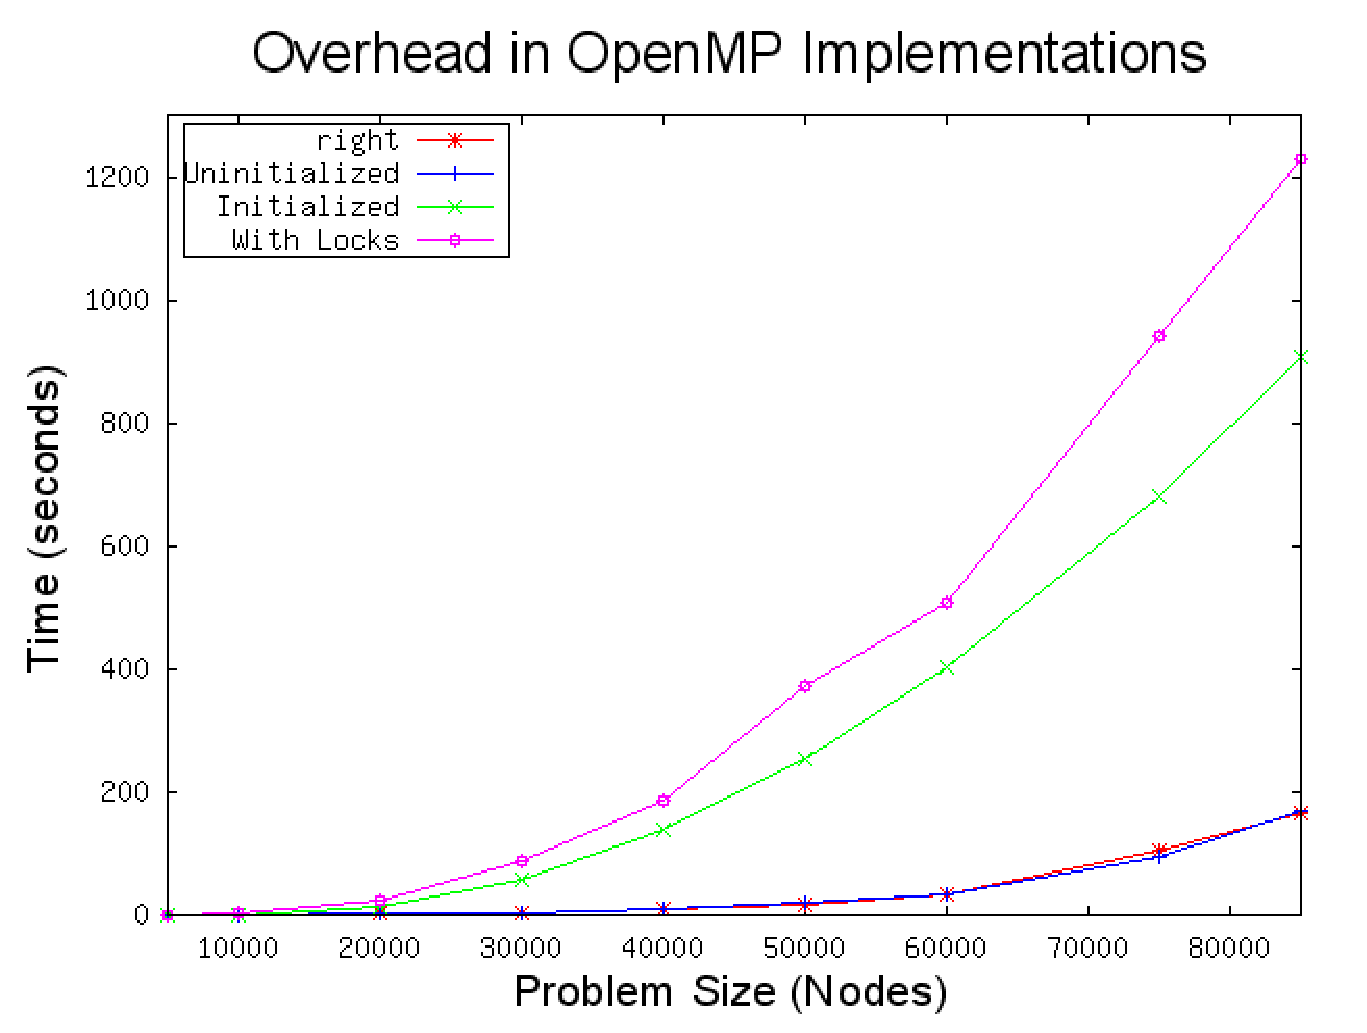
\includegraphics[width=0.25\textwidth]{images/figura1.eps}
\caption{Método de Kochanski}
\label{Kochanski}
\end{center}
\end{figure}


\section{Época moderna}
Desde el diseño de la primera computadora se empezaron a desarrollar programas para el cálculo del número \PI con la mayor cantidad de cifras
posible. De esta forma, en 1949 un ENIAC fue capaz de romper todos los récords, obteniendo 2037 cifras decimales en 70 horas. Poco a poco fueron
surgiendo ordenadores que batían récords y, de esta forma, pocos años después (1954) un NORAC llegó a 3092 cifras. Durante casi toda la década
de los años 1960 los IBM fueron batiendo récords, hasta que un IBM 7030 pudo llegar en 1966 a 250.000 cifras decimales (en 8 h y 23 min).
Durante esta época se probaban las nuevas computadoras con algoritmos para la generación de series de números procedentes de \PI, en la tabla \ref{tiempo},
podemos observar la evolución de las cifras.

\begin{table}[!ht]
\begin{center}
\begin{tabular}{|c|l|l|l|}
\hline
Año & Descubridor & Ordenador utilizado & Nº de cifras \\ \hline
1949 & G.W. Reitwiesner y otros & ENIAC & 2037 \\ \hline
1954 & & NORAC & 3092 \\ \hline
1959 & Guilloud & IBM 704 & 16167 \\ \hline
1967 & CDC & 6600 & 500000 \\ \hline
1973 & Guillord y Bouyer & CDC 7600 & 1001250 \\ \hline
1981 & Miyoshi y Kanada & FACOM M-200 & 2000036 \\ \hline
1982 & Guilloud & &	2000050 \\ \hline
\end{tabular}
\end{center}
\caption{Evolución del número de cifras}
\label{tiempo}
\end{table}














\bibliographystyle{plain}
\bibliography{bib/references}


\end{document}